% =====================================================================
% File        : 00_pengantar_matlab.tex
% Deskripsi   : Pengantar MATLAB untuk Makroekonomi, Bab 0 Intro: apa itu MATLAB, GNU Octave,
%               Dynare, lisensi dan biaya, penggunaan di fakultas
%               ekonomi, serta alasan MATLAB untuk DSGE dan tren ke
%               Python/Julia
% =====================================================================
\documentclass[aspectratio=169,11pt]{beamer}
\usetheme{metropolis}
\usepackage[utf8]{inputenc}
\usepackage{amsmath,amssymb}
\usepackage{booktabs}
\usepackage{array}
\newcolumntype{L}[1]{>{\raggedright\arraybackslash}p{#1}}
\usepackage{listings}
\usepackage{xurl}
\usepackage{tikz}
\usetikzlibrary{positioning,arrows.meta}

\definecolor{kolom}{RGB}{31,119,180}
\definecolor{baris}{RGB}{214,39,40}
\definecolor{kode}{RGB}{245,245,245}

\hypersetup{colorlinks=true, urlcolor=kolom, linkcolor=.}

\lstset{
  language=Matlab,
  basicstyle=\ttfamily\small,
  backgroundcolor=\color{kode},
  keywordstyle=\color{kolom}\bfseries,
  commentstyle=\color{gray}\itshape,
  frame=single, rulecolor=\color{gray!40},
  columns=fullflexible, keepspaces=true,
  xleftmargin=4pt, xrightmargin=4pt,
  showstringspaces=false
}

\lstdefinestyle{dynare}{
  language={},
  morekeywords={var,varexo,parameters,model,end,steady_state_model,
    initval,steady,check,shocks,stderr,stoch_simul,estimation,
    estimated_params,varobs},
  morecomment=[l]{//},
  keywordstyle=\color{kolom}\bfseries,
  commentstyle=\color{gray}\itshape
}

\title{Pengantar MATLAB untuk Makroekonomi}
\subtitle{Bab 0. Intro}
\author{Andreas Syaloom Kurniawan}
\institute{Faculty of Economics and Business, Universitas Gadjah Mada}
\date{}

\begin{document}

\maketitle

% ---------------------------------------------------------------------
\begin{frame}{Peta bab ini}
\small
\begin{enumerate}
  \item MATLAB itu aplikasi apa?
  \item Apakah sintaks GNU Octave sama dengan MATLAB?
  \item Apa itu Dynare, dan apakah bisa jalan di Octave?
  \item Desktop atau online? Berapa biayanya? Bisa gratis?
  \item MATLAB dipakai di fakultas ekonomi mana saja?
  \item Kenapa DSGE masih memakai MATLAB, bukan Python, R, atau Stata?
  \item Tren yang sedang bergeser: Python dan Julia
\end{enumerate}
\end{frame}

% =====================================================================
\section{MATLAB itu aplikasi apa?}
% =====================================================================

\begin{frame}{MATLAB = \textbf{MAT}rix \textbf{LAB}oratory}
\begin{itemize}
  \item Perangkat lunak komputasi numerik \emph{sekaligus} bahasa
        pemrograman, dikembangkan oleh \textbf{MathWorks}.
  \item Dirancang Cleve Moler (akhir 1970-an) sebagai antarmuka mudah ke
        pustaka aljabar linear LINPACK dan EISPACK; dikomersialkan
        tahun 1984.
  \item Ide utamanya: \alert{semua data adalah matriks atau array}.
        Satu angka pun sebenarnya matriks berukuran $1\times 1$.
  \item Bahasanya \emph{interpreted} dan \emph{high-level}: tidak perlu
        kompilasi, cocok untuk mencoba ide dengan cepat (\emph{prototyping}).
\end{itemize}
\end{frame}

% ---------------------------------------------------------------------
\begin{frame}[fragile]{Ide ``semua adalah matriks'' dalam praktik}
Mulai dari satu angka, lalu satu vektor. Operasinya ditulis dengan cara yang
sama.
\vspace{0.4em}
\begin{columns}[T]
\begin{column}{0.48\textwidth}
\begin{lstlisting}
x = 3;          % skalar (1x1)
y = 2*x + 1     % y = 7

v = [1 2 3];    % vektor (1x3)
w = 2*v + 1     % w = [3 5 7]
\end{lstlisting}
\end{column}
\begin{column}{0.48\textwidth}
\small
\begin{itemize}
  \item Rumus \texttt{2*x + 1} tidak berubah ketika \texttt{x} diganti
        vektor.
  \item Tidak perlu \emph{loop} untuk mengalikan setiap elemen.
  \item Gaya ini disebut \alert{vektorisasi}, dan menjadi ciri khas
        kode MATLAB yang baik.
\end{itemize}
\end{column}
\end{columns}
\end{frame}

% ---------------------------------------------------------------------
\begin{frame}{Dipakai untuk apa? (1) Teknik dan sains alam}
\footnotesize
\begin{columns}[T]
\begin{column}{0.32\textwidth}
\textbf{Teknik Kimia}
\begin{itemize}
  \item \textbf{Pemodelan dan simulasi proses:} model matematika reaktor
        kimia, perpindahan panas dan massa, serta aliran fluida, lalu
        disimulasikan.
  \item \textbf{Optimasi sistem:} mencari suhu, tekanan, atau laju alir
        optimal agar proses industri efisien dan hemat energi.
\end{itemize}
\end{column}
\begin{column}{0.32\textwidth}
\textbf{Teknik Mesin}
\begin{itemize}
  \item \textbf{Simulasi sistem dinamis dan kontrol:} Simulink untuk
        sistem kendali otomatis, suspensi kendaraan, atau dinamika motor.
  \item \textbf{Optimasi desain:} mencari efisiensi atau kekuatan terbaik
        struktur mesin sebelum fabrikasi atau uji prototipe.
\end{itemize}
\end{column}
\begin{column}{0.32\textwidth}
\textbf{Teknik Elektro}
\begin{itemize}
  \item \textbf{Sistem kendali:} merancang dan menganalisis kestabilan
        sistem otomatis atau kontrol motor (Simulink).
  \item \textbf{Sinyal dan telekomunikasi:} filter, transformasi Fourier,
        analisis spektral, simulasi komunikasi digital.
  \item \textbf{Citra dan video:} citra digital, citra medis, hingga
        AI/\emph{deep learning}.
\end{itemize}
\end{column}
\end{columns}
\end{frame}

% ---------------------------------------------------------------------
\begin{frame}{Dipakai untuk apa? (2) Ekonomi dan keuangan}
\footnotesize
\begin{columns}[T]
\begin{column}{0.38\textwidth}
\textbf{Makroekonomi}
\begin{itemize}
  \item Model DSGE (lewat \textbf{Dynare})
  \item Estimasi VAR/SVAR
  \item Optimisasi dan simulasi numerik
\end{itemize}
\vspace{0.4em}
\textbf{Keuangan: portofolio dan risiko}
\begin{itemize}
  \item \textbf{Optimasi portofolio:} analisis, \emph{backtesting}, dan
        optimasi dengan biaya transaksi, batasan aset, serta rasio risiko.
  \item \textbf{Manajemen risiko:} risiko pasar, \emph{credit scorecard}
        perbankan, dan uji stres portofolio besar.
\end{itemize}
\end{column}
\begin{column}{0.58\textwidth}
\textbf{Keuangan: pricing dan pemodelan}
\begin{itemize}
  \item \textbf{Valuasi instrumen:} harga obligasi, swap, opsi Eropa/Amerika,
        dan derivatif kompleks dengan Monte Carlo atau Black--Scholes.
  \item \textbf{Kurva imbal hasil:} kurva suku bunga dan inflasi, serta
        pencocokan model seperti Nelson--Siegel.
  \item \textbf{Time series finansial:} data historis maupun
        \emph{real-time}, penanganan data hilang, dan konversi kalender
        perdagangan.
  \item \textbf{Proses stokastik:} pergerakan harga atau suku bunga dengan
        persamaan diferensial stokastik.
\end{itemize}
\end{column}
\end{columns}
\end{frame}

% ---------------------------------------------------------------------
\begin{frame}[fragile]{Ekosistem MATLAB: inti, toolbox, Simulink, pihak ketiga}
\begin{columns}[T]
\begin{column}{0.42\textwidth}
\centering
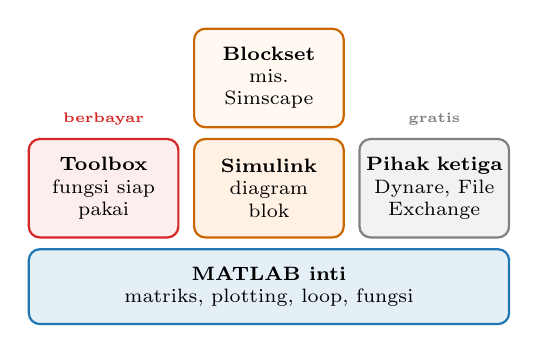
\begin{tikzpicture}[
  lapis/.style={draw, thick, rounded corners, align=center, font=\scriptsize,
                inner sep=2pt},
  atas/.style={lapis, minimum width=1.9cm, text width=1.75cm,
               minimum height=1.25cm}]
\node[lapis, draw=kolom, fill=kolom!12, minimum width=6.1cm,
      minimum height=0.95cm] (inti) at (0,0)
  {\textbf{MATLAB inti}\\matriks, plotting, loop, fungsi};
\node[atas, draw=baris, fill=baris!8] (tb) at (-2.1,1.25)
  {\textbf{Toolbox}\\fungsi siap\\pakai};
\node[atas, draw=orange!80!black, fill=orange!10] (sl) at (0,1.25)
  {\textbf{Simulink}\\diagram\\blok};
\node[atas, draw=gray, fill=gray!10] (pk) at (2.1,1.25)
  {\textbf{Pihak ketiga}\\Dynare, File\\Exchange};
\node[atas, draw=orange!80!black, fill=orange!5] (bs) at (0,2.65)
  {\textbf{Blockset}\\mis.\\\mbox{Simscape}};
\node[font=\tiny\bfseries, text=baris, above=1pt of tb] {berbayar};
\node[font=\tiny\bfseries, text=gray, above=1pt of pk] {gratis};
\end{tikzpicture}

\vspace{0.4em}
\raggedright\scriptsize
Semua lapisan atas \alert{membutuhkan MATLAB inti} untuk berjalan.
\end{column}
\begin{column}{0.56\textwidth}
\scriptsize
\textbf{Toolbox} = kumpulan fungsi tambahan untuk satu bidang,
dipakai lewat kode seperti biasa.
\begin{itemize}
  \item Optimization: \texttt{fmincon}, \texttt{fminunc};
        Econometrics: \texttt{varm}, \texttt{garch};
        Financial: optimasi portofolio, valuasi obligasi.
  \item \alert{Mirip library Python atau package R}, tetapi resmi dari
        MathWorks, \textbf{berbayar}, dan terikat lisensi: kode yang memakai
        toolbox tidak jalan di komputer tanpa lisensi toolbox itu.
\end{itemize}
\textbf{Simulink} = aplikasi grafis tersendiri. Model disusun dengan
menyeret dan menghubungkan \emph{blok}, lalu disimulasikan sepanjang waktu.
\begin{itemize}
  \item Umum di teknik; jarang di ekonomi, karena DSGE ditulis sebagai
        persamaan (Dynare), bukan diagram.
\end{itemize}
\textbf{Pihak ketiga} = kode di luar MathWorks yang ditambahkan ke
\emph{path}, seperti Dynare atau kiriman pengguna di File Exchange.
Gratis, paling mirip budaya \texttt{pip install}.
\end{column}
\end{columns}
\end{frame}

% ---------------------------------------------------------------------
\begin{frame}{Kelemahan dan alternatif}
\textbf{Kelemahan MATLAB:} proprietary, lisensi inti dan tiap toolbox
berbayar, dan kode sumber sebagian tertutup.
\vspace{0.6em}

\centering\small
\renewcommand{\arraystretch}{1.2}
\begin{tabular}{L{3.4cm} L{4.8cm} L{4.4cm}}
\toprule
Alternatif & Kelebihan & Catatan \\
\midrule
\textbf{GNU Octave} & Gratis, sintaks hampir sama, jalan Dynare & Lebih lambat untuk loop \\
Python (NumPy/SciPy) & Gratis, ekosistem sangat luas & Belum ada padanan Dynare yang matang \\
Julia & Gratis, cepat, sintaks mirip MATLAB & Ekosistem lebih kecil \\
\bottomrule
\end{tabular}
\end{frame}

% =====================================================================
\section{Apakah sintaks GNU Octave sama dengan MATLAB?}
% =====================================================================

\begin{frame}[fragile]{Jawaban singkat: sebagian besar sama}
GNU Octave adalah perangkat lunak \alert{gratis dan open source} yang
sengaja dirancang agar kompatibel dengan MATLAB. Kode umum seperti ini jalan
di keduanya tanpa diubah:
\vspace{0.3em}
\begin{lstlisting}
A = [2 1; 1 3];             % matriks 2x2
b = [1; 2];                 % vektor kolom
x = A \ b;                  % selesaikan sistem Ax = b
for i = 1:3
    fprintf('Iterasi ke-%d\n', i);
end
plot(1:10, (1:10).^2)       % grafik sederhana
\end{lstlisting}
\small Operasi matriks, \texttt{for}/\texttt{if}/\texttt{while}, file fungsi,
\texttt{fprintf}, indexing, dan plotting dasar: semuanya sama.
\end{frame}

% ---------------------------------------------------------------------
\begin{frame}[fragile]{Octave lebih longgar: sintaks yang hanya jalan di Octave}
\centering\small
\renewcommand{\arraystretch}{1.15}
\begin{tabular}{l l l}
\toprule
Fungsi & Hanya di Octave & Portabel (MATLAB \& Octave) \\
\midrule
Komentar        & \texttt{\# komentar}      & \texttt{\% komentar} \\
Tidak sama dengan & \texttt{!=}             & \texttt{\textasciitilde=} \\
Negasi          & \texttt{!a}               & \texttt{\textasciitilde a} \\
Penugasan majemuk & \texttt{x += 1}         & \texttt{x = x + 1} \\
Increment       & \texttt{x++}              & \texttt{x = x + 1} \\
Penutup blok    & \texttt{endif}, \texttt{endfor} & \texttt{end} \\
Cetak           & \texttt{printf(...)}      & \texttt{fprintf(...)} \\
\bottomrule
\end{tabular}

\vspace{0.8em}
\raggedright
\alert{Aturan praktis:} selalu tulis dengan gaya MATLAB (kolom kanan).
Kode seperti itu jalan di kedua aplikasi.
\end{frame}

% ---------------------------------------------------------------------
\begin{frame}{Perbedaan yang perlu diwaspadai}
\begin{enumerate}
  \item \textbf{Tanda kutip ganda.} Di Octave, \texttt{"..."} adalah
        \emph{char array} biasa yang memproses \emph{escape} (\texttt{\textbackslash n}).
        Di MATLAB (sejak R2017a), \texttt{"..."} membuat objek
        \texttt{string}, tipe yang berbeda dari \texttt{'...'}.
        Sumber bug yang sering muncul.
  \item \textbf{Fitur yang tidak ada atau terbatas di Octave.}
        Simulink dan App Designer tidak ada; \texttt{classdef} parsial;
        \texttt{table}, \texttt{datetime}, dan blok \texttt{arguments}
        belum (sepenuhnya) didukung.
  \item \textbf{Toolbox vs packages.} Toolbox MATLAB diganti
        \emph{packages} Octave (\texttt{statistics}, \texttt{optim},
        \texttt{signal}); nama fungsi dan cakupannya tidak selalu sama.
  \item \textbf{Kecepatan.} MATLAB punya \emph{JIT compiler}, sehingga loop
        jauh lebih cepat. Di Octave, loop bisa sangat lambat, jadi
        vektorisasi makin penting.
\end{enumerate}
\end{frame}

% =====================================================================
\section{Apa itu Dynare?}
% =====================================================================

\begin{frame}{Dynare: platform untuk model ekonomi dinamis}
\begin{itemize}
  \item Perangkat lunak \alert{open source} (GPL) untuk menyelesaikan,
        mensimulasikan, dan mengestimasi model ekonomi dinamis, terutama
        \textbf{DSGE} dan juga model OLG.
  \item Dikembangkan tim di \textbf{CEPREMAP}, Paris; pengembang awalnya
        Michel Juillard.
  \item Dynare \emph{bukan} aplikasi berdiri sendiri: ia menumpang di
        \textbf{MATLAB} atau \textbf{GNU Octave}.
\end{itemize}
\vspace{0.6em}
\centering
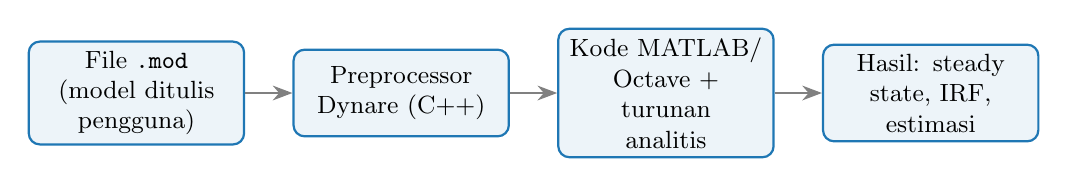
\begin{tikzpicture}[
  kotak/.style={draw=kolom, thick, rounded corners, fill=kolom!8,
                align=center, minimum height=1.1cm, text width=2.5cm,
                font=\small},
  panah/.style={-{Stealth[length=2.5mm]}, thick, gray}]
\node[kotak] (mod) {File \texttt{.mod}\\(model ditulis\\pengguna)};
\node[kotak, right=0.6cm of mod] (pre) {Preprocessor\\Dynare (C++)};
\node[kotak, right=0.6cm of pre] (kode) {Kode MATLAB/\\Octave + turunan\\analitis};
\node[kotak, right=0.6cm of kode] (hasil) {Hasil: steady\\state, IRF,\\estimasi};
\draw[panah] (mod) -- (pre);
\draw[panah] (pre) -- (kode);
\draw[panah] (kode) -- (hasil);
\end{tikzpicture}
\end{frame}

% ---------------------------------------------------------------------
\begin{frame}[fragile]{Seperti apa file \texttt{.mod}? Kerangka blok-bloknya}
\begin{columns}[T]
\begin{column}{0.5\textwidth}
\begin{lstlisting}[style=dynare,basicstyle=\ttfamily\scriptsize]
var y c k;              // endogen
varexo e;               // shock
parameters alpha beta;
alpha = 0.33;  beta = 0.99;
model;
  // persamaan model di sini
end;
steady_state_model;
  // solusi steady state
end;
shocks; var e; stderr 0.01; end;
stoch_simul(order=1);
\end{lstlisting}
\end{column}
\begin{column}{0.46\textwidth}
\small
Urutan logisnya mengikuti cara kita menulis model di kertas:
\begin{enumerate}
  \item Deklarasikan variabel endogen, shock, dan parameter.
  \item Beri nilai parameter (kalibrasi).
  \item Tulis persamaan model.
  \item Berikan steady state.
  \item Tentukan ukuran shock.
  \item Minta Dynare menghitung: di sini simulasi stokastik orde 1
        (\texttt{stoch\_simul}).
\end{enumerate}
\end{column}
\end{columns}
\end{frame}

% ---------------------------------------------------------------------
\begin{frame}{Apa saja yang bisa dikerjakan Dynare?}
\begin{columns}[T]
\begin{column}{0.48\textwidth}
\textbf{Solusi dan simulasi}
\begin{itemize}\small
  \item Penghitungan steady state
  \item Solusi perturbasi orde 1, 2, 3, dan lebih tinggi
  \item Simulasi deterministik (\emph{perfect foresight})
  \item \emph{Occasionally binding constraints} (OccBin), mis.\ ZLB
\end{itemize}
\end{column}
\begin{column}{0.48\textwidth}
\textbf{Estimasi dan kebijakan}
\begin{itemize}\small
  \item Estimasi Bayesian (Metropolis--Hastings)
  \item Maximum likelihood
  \item Analisis identifikasi parameter
  \item Kebijakan optimal: Ramsey dan \emph{discretion}
\end{itemize}
\end{column}
\end{columns}
\end{frame}

% ---------------------------------------------------------------------
\begin{frame}{Apakah Dynare bisa jalan di Octave?}
\textbf{Ya, resmi didukung.} Setiap rilis Dynare mencantumkan versi Octave
yang kompatibel di halaman unduhannya. Catatan praktis:
\vspace{0.3em}
\begin{enumerate}
  \item \textbf{Kecepatan.} Estimasi Bayesian dengan rantai MCMC panjang
        bisa jauh lebih lambat di Octave.
  \item \textbf{Optimizer.} Beberapa opsi \texttt{mode\_compute} memanggil
        Optimization Toolbox MATLAB (\texttt{fmincon}, \texttt{fminunc}).
        Di Octave: pasang package \texttt{optim}, atau pakai optimizer bawaan
        Dynare (\texttt{mode\_compute=4} csminwel, atau \texttt{mode\_compute=6}).
  \item \textbf{Dokumentasi.} Mayoritas pengguna dan contoh di forum memakai
        MATLAB, sehingga masalah khusus Octave lebih jarang dibahas.
\end{enumerate}
\vspace{0.3em}
\alert{Kesimpulan:} untuk model kecil sampai menengah, Octave sudah sangat
memadai. Ada juga \textbf{Dynare.jl} untuk Julia, meski fiturnya belum
selengkap versi MATLAB/Octave.
\end{frame}

% =====================================================================
\section{Versi, biaya, dan akses gratis}
% =====================================================================

\begin{frame}{Desktop atau online? Keduanya.}
\begin{columns}[T]
\begin{column}{0.48\textwidth}
\textbf{MATLAB Desktop}
\begin{itemize}\small
  \item Diinstal di Windows, macOS, atau Linux
  \item Memakai CPU dan memori komputer sendiri
  \item Cocok untuk estimasi berat yang berjalan lama
\end{itemize}
\end{column}
\begin{column}{0.48\textwidth}
\textbf{MATLAB Online}
\begin{itemize}\small
  \item Dijalankan lewat browser, server milik MathWorks
  \item File tersimpan di MATLAB Drive
  \item Tidak perlu instalasi; bisa dari komputer mana pun
\end{itemize}
\end{column}
\end{columns}
\vspace{0.8em}
Dengan lisensi berbayar atau lisensi kampus, biasanya Anda mendapat akses ke
\alert{dua-duanya}.
\end{frame}

% ---------------------------------------------------------------------
\begin{frame}{Biaya lisensi (per Oktober 2026)}
\centering\small
\renewcommand{\arraystretch}{1.2}
\begin{tabular}{l l l l}
\toprule
Lisensi & Harga & Isi & Siapa yang boleh \\
\midrule
Student  & US\$119/tahun & MATLAB, Simulink, 11 toolbox & Mahasiswa aktif \\
Home     & US\$165/tahun & MATLAB + 12 toolbox & Pribadi, non-komersial \\
Standard & $\pm$US\$940/tahun* & MATLAB saja (toolbox terpisah) & Komersial, pemerintah \\
\bottomrule
\end{tabular}

\vspace{0.7em}
\raggedright\footnotesize
\begin{itemize}
  \item Sejak 1 Januari 2026, lisensi \emph{perpetual} Student dan Home
        dihentikan dan diganti langganan tahunan; MATLAB saja (tanpa paket)
        tidak bisa lagi dibeli untuk kedua kategori itu.
  \item *Angka Standard dari sumber pihak ketiga (2025). Semua harga belum
        termasuk pajak; cek toko MathWorks untuk wilayah Indonesia.
\end{itemize}
\end{frame}

% ---------------------------------------------------------------------
\begin{frame}{Mau gratis? Bisa, ada empat jalur}
\begin{enumerate}
  \item \textbf{Lisensi kampus (Campus-Wide License).} Jalur terbaik.
        Buat akun MathWorks dengan email institusi (mis.\
        \texttt{@mail.ugm.ac.id}); jika kampus berlangganan, akun otomatis
        tertaut ke lisensi. Jika ragu, tanyakan ke unit TI kampus.
  \item \textbf{MATLAB Online (basic).} Gratis 20 jam per bulan, akses ke
        10 produk umum, komputasi kontinu maksimal 15 menit, penyimpanan
        5 GB. Cukup untuk latihan, \alert{tidak} untuk estimasi DSGE yang lama.
  \item \textbf{Trial 30 hari.} Desktop dan online tanpa batas selama
        30 hari, termasuk MATLAB, Simulink, dan 80+ produk.
  \item \textbf{GNU Octave.} Gratis selamanya dan bisa menjalankan Dynare.
\end{enumerate}
\end{frame}

% ---------------------------------------------------------------------
\begin{frame}{Catatan penting soal penggunaan lisensi}
\begin{itemize}
  \item Lisensi \textbf{Student} dan \textbf{Home} sama-sama
        \alert{melarang} penggunaan untuk pekerjaan berbayar atau untuk
        organisasi.
  \item Lisensi Home secara eksplisit juga tidak untuk keperluan
        pemerintah dan akademik.
\end{itemize}
\vspace{0.6em}
\centering\small
\renewcommand{\arraystretch}{1.2}
\begin{tabular}{l l}
\toprule
Kegiatan & Lisensi yang sesuai \\
\midrule
Tugas kuliah, tesis, disertasi & Student atau lisensi kampus \\
Belajar pribadi di rumah & Home atau Octave \\
Proyek kajian untuk instansi/klien & Standard, lisensi institusi, atau Octave \\
\bottomrule
\end{tabular}
\end{frame}

% =====================================================================
\section{MATLAB di fakultas ekonomi}
% =====================================================================

\begin{frame}{Contoh mata kuliah ekonomi yang memakai MATLAB}
\footnotesize
\renewcommand{\arraystretch}{1.25}
\begin{tabular}{L{2.9cm} L{4.1cm} L{5.4cm}}
\toprule
Kampus & Mata kuliah & Isi singkat \\
\midrule
University of Florida, AS &
ECO 7938 Practical Computing in Economics &
R di paruh pertama semester, MATLAB di paruh kedua \\
University of Konstanz, Jerman &
Programming for Economics (B.Sc.) &
Dasar pemrograman untuk ekonomi; seluruh aplikasi memakai MATLAB \\
Università di Roma Tor Vergata, Italia &
Mata kuliah MATLAB, M.Sc.\ Economics &
Pengantar MATLAB, lalu estimasi ARMA, VAR, dan EC \\
Université Paris Dauphine-PSL, Prancis &
Introduction to Matlab programming (M1 Quantitative Economics) &
Matriks, plotting, loop, fungsi, optimisasi dasar untuk data dan model ekonomi \\
\bottomrule
\end{tabular}
\end{frame}

% ---------------------------------------------------------------------
\begin{frame}{Tautan silabus}
\footnotesize
\begin{description}[Tor Vergata]
  \item[Florida] \url{https://economics.clas.ufl.edu/wp-content/uploads/sites/117/ECO7938_Heins_F22.pdf}
  \item[Konstanz] \url{https://www.wiwi.uni-konstanz.de/}
        \\ (silabus PDF ada di situs Departemen Ekonomi)
  \item[Tor Vergata] \url{https://economia.uniroma2.it/master-science/economics/corso/426/}
  \item[Dauphine] \url{https://preview.offre.dauphine.fr/cdm/fr-FR/fiche/M5SAN/programme/4MQUEP01}
        \\ \url{https://dauphine.psl.eu/fileadmin/mediatheque/formations/masters/quantitative-economics/m2-analysis/Compendium_of_M1_syllabus_2025-2026.pdf}
\end{description}
\end{frame}

% =====================================================================
\section{Kenapa DSGE masih memakai MATLAB?}
% =====================================================================

\begin{frame}{Lima alasan utama}
\begin{enumerate}
  \item \textbf{Dynare adalah standar de facto}, dan Dynare lahir di MATLAB.
        Python belum punya padanan yang setara kematangannya.
  \item \textbf{Replikasi dan model bank sentral.} Kode replikasi paper
        DSGE klasik (Smets--Wouters 2007, Christiano--Eichenbaum--Evans 2005)
        dan banyak model bank sentral tersedia di MATLAB/Dynare
        (tautan di slide berikut).
  \item \textbf{Cocok secara teknis.} Inti solusi DSGE adalah aljabar linear:
        dekomposisi QZ, filter Kalman, MCMC. MATLAB dibangun di atas
        LAPACK/BLAS, dan JIT-nya membuat loop cukup cepat.
  \item \textbf{Inersia pengajaran.} Dosen makro generasi sekarang dilatih
        dengan MATLAB, dan lisensi kampus membuat biaya bagi mahasiswa nol.
  \item \textbf{Stabilitas.} Kode MATLAB berumur 15 tahun umumnya masih jalan;
        penting untuk replikasi jangka panjang.
\end{enumerate}
\end{frame}

% ---------------------------------------------------------------------
\begin{frame}{Tautan kode replikasi DSGE klasik}
\scriptsize
\setlength{\itemsep}{0pt}
\textbf{Smets dan Wouters (2007), \emph{American Economic Review}}
\begin{itemize}
  \item Paket replikasi resmi AER (kode dan data asli):
        \\ \url{https://www.aeaweb.org/aer/data/june07/20041254_data.zip}
  \item Versi Dynare yang diperbarui (Johannes Pfeifer):
        \\ \url{https://github.com/JohannesPfeifer/DSGE_mod/blob/master/Smets_Wouters_2007/Smets_Wouters_2007_45.mod}
\end{itemize}
\textbf{Christiano, Eichenbaum, dan Evans (2005), \emph{Journal of Political Economy}}
\begin{itemize}
  \item Replikasi Dynare dari komunitas (Forum Dynare, 2009):
        \\ \url{https://archives.dynare.org/phpBB3/viewtopic.php\%3Fp=4140.html}
  \item Catatan: kode asli CEE tidak ditulis di Dynare; versi Dynare
        adalah rekonstruksi pengguna.
\end{itemize}
\textbf{Macroeconomic Model Data Base (MMB)}
\begin{itemize}
  \item Arsip 160+ model makro struktural dalam format Dynare, termasuk
        SW07, varian Christiano dkk., dan model bank sentral (mis.\ NAWM
        ECB, model proyeksi IMF): \url{https://www.macromodelbase.com}
\end{itemize}
\end{frame}

% ---------------------------------------------------------------------
\begin{frame}{Kenapa bukan R atau Stata?}
R dan Stata dirancang untuk \alert{statistik dan ekonometrika}, bukan untuk
menyelesaikan sistem persamaan dinamis dengan ekspektasi rasional.
\vspace{0.3em}

\centering\footnotesize
\renewcommand{\arraystretch}{1.05}
\begin{tabular}{L{2.3cm} L{3.6cm} L{6.4cm}}
\toprule
Alat & Unggul untuk & Untuk DSGE \\
\midrule
Stata & Mikroekonometrika, data panel & \texttt{dsge}/\texttt{dsgenl}: hanya linearisasi orde 1, model kecil \\
R & Statistik, VAR/SVAR, visualisasi & Praktis tidak ada ekosistem serius \\
Python & Data, machine learning, umum & Ada (gEconpy, pydsge, dolo), belum sematang Dynare \\
MATLAB + Dynare & Model struktural & Lengkap: orde tinggi, Bayesian, OccBin, Ramsey \\
\bottomrule
\end{tabular}

\vspace{0.4em}
\raggedright\footnotesize
Untuk VAR/SVAR dan deret waktu, R dan Stata memadai; untuk keseimbangan umum
struktural, bukan alat yang tepat.
\end{frame}

% =====================================================================
\section{Tren yang sedang bergeser}
% =====================================================================

\begin{frame}{Garis depan riset makro bergerak ke Python dan Julia}
\begin{columns}[T]
\begin{column}{0.5\textwidth}
\textbf{Kenapa bergeser?}
\begin{itemize}\small
  \item Riset makro kini banyak memakai model \textbf{agen heterogen}
        (HANK), di mana Dynare kurang unggul.
  \item Alat paling berpengaruh untuk HANK, \emph{Sequence-Space Jacobian}
        toolkit (Auclert, Bardóczy, Rognlie, Straub), ditulis dalam
        \textbf{Python}.
  \item \textbf{Julia}: secepat bahasa terkompilasi, sintaks mirip MATLAB,
        gratis. Ekosistem QuantEcon, dolo, dan Dynare.jl.
\end{itemize}
\end{column}
\begin{column}{0.46\textwidth}
\textbf{Contoh di Paris}
\begin{itemize}\small
  \item \textbf{ENSAE (IP Paris)}: metode numerik makro diajarkan dengan
        \alert{Julia}.
  \item \textbf{Paris 1 Panthéon-Sorbonne}: DSGE di Master in Economics
        dipraktikkan dengan \alert{Python}.
  \item \textbf{Dauphine-PSL, PSE, Bordeaux}: masih MATLAB/Dynare.
\end{itemize}
\end{column}
\end{columns}
\end{frame}

% ---------------------------------------------------------------------
\begin{frame}{Ringkasan}
\begin{itemize}
  \item MATLAB adalah lingkungan komputasi berbasis matriks; GNU Octave
        adalah alternatif gratis dengan sintaks hampir sama.
  \item Dynare adalah standar untuk DSGE dan jalan di MATLAB maupun Octave.
  \item Akses gratis: lisensi kampus, MATLAB Online (basic), trial,
        atau Octave. Perhatikan batasan lisensi Student/Home.
  \item MATLAB masih dominan untuk DSGE agen representatif karena ekosistem
        Dynare, replikasi, dan inersia pengajaran.
  \item Untuk riset makro komputasi mutakhir (HANK), pusat gravitasinya
        mulai pindah ke \alert{Python dan Julia}.
\end{itemize}
\vspace{0.4em}
\small Bab-bab berikutnya memakai sintaks MATLAB yang portabel, sehingga
semua contoh juga bisa dijalankan di Octave.
\end{frame}

% ---------------------------------------------------------------------
\begin{frame}{Sumber}
\scriptsize
\begin{itemize}
  \item MATLAB Online (basic) dan batasannya:
        \url{https://au.mathworks.com/products/matlab-online/matlab-online-versions.html}
  \item Trial 30 hari: \url{https://www.mathworks.com/trials/}
  \item Perubahan lisensi Student/Home 2026 (MATLAB Central):
        \url{https://in.mathworks.com/matlabcentral/discussions?view=full}
  \item Ketentuan lisensi Home: \url{https://jp.mathworks.com/pricing-licensing.html}
  \item Harga Standard (pihak ketiga): \url{https://www.thepricer.org/how-much-does-matlab-license-cost/}
  \item Dynare di NumFOCUS: \url{https://numfocus.org/project/dynare}
  \item Daftar model MMB: \url{https://www.macromodelbase.com/files/documentation_source/mmb-model-description.pdf}
  \item ENSAE, Macroeconomics 2: \url{https://ensae.fr/en/courses/600}
  \item Paris 1, Macroeconomics: \url{https://cours.univ-paris1.fr/course/view.php?id=39728}
  \item Situs resmi Dynare: \url{https://www.dynare.org}
\end{itemize}
\end{frame}

\end{document}
